\chapter{Methods}
\label{ch:whatYouDid}

\com{
\todo[inline]{Choose your own chapter title to describe this}

\todo[inline]{What have you done? How did you do it? What design decisions did you make? How did what you did help you to meet your goals?}
}



\subsection{Robotic Operating System Framework}
\label{ssec:ros}
\noindent \Gls{ROS}\cite{288} is an open-source framework, and not an actual operating system, widely adopted for building software used to control robotic systems.
\Gls{ROS} works both with C++ and Python programmed scripts, allowing for developers with different backgrounds to develop upon it.

During the past decade it has seen numerous improvements by the community and it provides a collection of several libraries, tools, and conventions made to simplify the modular creation and interaction of complex robotic systems.
Its modular structure is composed by available packages containing well-debugged code which can be adapted and run together with newly made packages built to satisfy the projects requirements.
These packages are composed by modules of software which can be described as custom nodes, libraries, processes, and messages.
A robotic system operates using an interconnection of different nodes which have just minimal tasks to execute.
Its services are mostly developed as a middle-layer infrastructure to allow for interaction of heterogeneous devices, ranging from low-level device control to embedded system, providing hardware abstraction and enabling message-passing between processes.

For these nodes to cooperate, they are connected by a middle-layer structure based on a network of topics or services, following a blackboard architecture of data sharing.
It provides a graph-like structure were each program, described as node, can both publish and subscribe messages among the created and available topics.
Topics can be seen as variables which are used for streaming communication and share information between nodes.
A \Gls{ROS} node publishes a specific message through a topic and every other node can subscribe to that topic and receive all the messages posted to it.
A \Gls{ROS} system, to behave as expected, needs a master process which has the task of matching publishers and subscribers to their related topics.
These topics can be generated by sensors, actuators, planners, controllers of different kind and made available using this structure of topics, similar to a blackboard architecture.
Each topic is defined by a specific message type which specifies its content in order to standardise its usage among applications and to simplify communication between nodes.
Messages definition can be customised and they are stored inside the \Gls{ROS} package, defining the data sent within the topic which will use that definition.
Figure \ref{fig:ros-topic} shows an example of a \Gls{ROS} graph where two subscriber nodes receive the messages posted on the topic by a publisher node.

\begin{figure}[!ht]
	%\textbf{Investigating Simultaneous Localization and Mapping for AGV systems}
	\begin{center}
		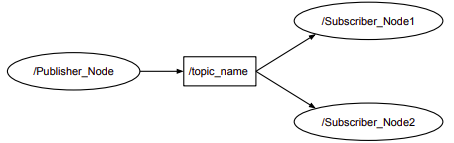
\includegraphics[width=0.75\textwidth]{Images/2-Background/ROSTopic-2021-04-22 10-51-37.png}
	\end{center}
	\caption{Example of \Gls{ROS} architecture for information sharing\cite{palsson_investigating_2017}}
	\label{fig:ros-topic}
\end{figure}

The aspect of localisation is important for the robotics field, to understand where the robot is located with respect to the rest of the world, but also to know how the sensors are positioned with respect to the robot in which they are installed.
It is of prominent importance to be aware of the different pose of the connected sensors before fusing their information, as the measurements of each sensors are related to their specific coordinate frame.
Before performing sensors fusion, every different frames of the sensors need to be transformed into the base frame of the robot which they are measuring to be sure about that the measurements refers to the same coordinate frame.
\Gls{ROS} uses the TF\cite{6556373} library to provide the tools needed to work with coordinate frames and to deal with their related transformation.
It allows for the definition of each sensor rigid body transform to specify their related position with respect to the robot, and then the library will deal with all the other transformations by publishing messages regarding to the rotational and translational relations between frames.
Commonly used frames are odom and base\_link, as shown in figure \ref{fig:ros-frames}. The odom frame has the origin at the initial position $P_{odom}$ of the robot and it is used to keep track of its moving behaviour. The base\_link frame is rigidly attached to the robot base $P_{base}$ and it is used to define the frames of its attached components. A transformation to map the the base\_link frame into the odom frame in \Gls{2D} with a rotation along the Z axis of $\theta$ and with a translation of $(x',y')$ is defined using an orthogonal matrix as in equation \ref{eq:transf}:
\begin{align}
	P_{odom} = T^o_b \cdot P_{base} && \textrm{where} ~
	T^o_b =
	\begin{bmatrix}
		cos(\theta) & -sin(\theta) & x' \\
		sin(\theta) & cos(\theta) & y' \\
		0 & 0 & 1 \\
	\end{bmatrix}
	\label{eq:transf}
\end{align}


\begin{figure}[!ht]
	%\textbf{Investigating Simultaneous Localization and Mapping for AGV systems}
	\begin{center}
		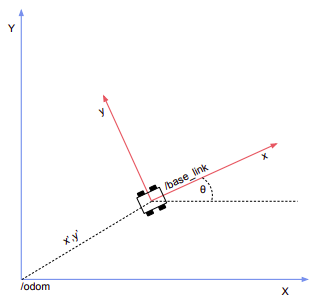
\includegraphics[width=0.5\textwidth]{Images/2-Background/Frames-2021-04-22 12-03-22.png}
	\end{center}
	\caption{Example of relation between \Gls{ROS} frames.\cite{palsson_investigating_2017}}
	\label{fig:ros-frames}
\end{figure}

Describe the engineering-related contents (preferably with models) and the research methodology and methods that are used in the degree project.

Give a theoretical description of the scientific or engineering methodology are you going to use and why have you chosen this method. What other methods did you consider and why did you reject them.

In this chapter, you describe what engineering-related and scientific skills you are going to apply, such as modeling, analyzing, developing, and evaluating engineering-related and scientific content. The choice of these methods should be appropriate for the problem . Additionally, you should be consciousness of aspects relating to society and ethics (if applicable). The choices should also reflect your goals and what you (or someone else) should be able to do as a result of your solution - which could not be done well before you started.

The purpose of this chapter is to provide an overview of the research method
used in this thesis. Section~\ref{sec:researchProcess} describes the research
process. Section~\ref{sec:researchParadigm} details the research
paradigm. Section~\ref{sec:dataCollection} focuses on the data collection
techniques used for this research. Section~\ref{sec:experimentalDesign}
describes the experimental design. Section~\ref{sec:assessingReliability}
explains the techniques used to evaluate the reliability and validity of the
data collected. Section~\ref{sec:plannedDataAnalysis} describes the method
used for the data analysis. Finally, Section~\ref{sec:evaluationFramework}
describes the framework selected to evaluate xxx.


\section{Research Process}
\label{sec:researchProcess}

\com{
\begin{figure}[!ht]
  \begin{center}
    \includegraphics[width=0.5\textwidth]{Images/4-Done/}
  \end{center}
  \caption{Research Process}
  \label{fig:researchprocess}
\end{figure}
}

\section{Research Paradigm}
\label{sec:researchParadigm}

\section{Data Collection}
\todo[inline]{This should also show that you are aware of the social and ethical concerns that might be relevant to your data collection method.)}
\label{sec:dataCollection}
To gather data used to test and analyse the performance of the system, multiple outdoor tests have been carried on.
Some tests have been made to define the calibration of the sensors against a ground truth identified using measure tape.
Some other tests have been made to ensure that the system is behaving accurately while steering.
Some tests have been made to check that the collision events are estimated with an certain degree of precision.

During these tests the rosbag utils provided by ROS has been exploited. Through this service it is possible to store every message sent to the topics, and they can be reused in the future to tune the algorithms.
In this way, the real measurements gathered during outdoor testing can be re evaluated through the play of said messages and using a simulated parameter to reset the clock of ROS framework.



\subsection{Sampling}


\section{Experimental design / Planned Measurements}
\label{sec:experimentalDesign}

\subsection{Test environment / test bed / model}\todo[inline]{Describe everything that someone else would need to reproduce your test environment/test bed/model/… .}

\subsection{Hardware / Software to be used}
Raspberry Pi 4 to guide the automower, to gather information about the topics of ROS, and to communicate them to the personal computer used to gather them.
Husqvarna Automower that holds the sensors and the raspberry pi, also proving the measurements of the wheel encoders and of the embedded GPS receiver.
Computer to guide the automower and make him move according to the desired path, also at the end the automower was free to run its random path and use the algorithm implemented to stay inside the boundaries.


\section{Assessing reliability and validity of the data collected}
\label{sec:assessingReliability}
Test on real measurements gathered in different conditions of terrain, slope, and conditions.
Multiple tests have been repeated to measure the measurement's value noise of each sensors.


\subsection{Validity of method}
\todo[inline]{How will you know if your results are valid?}

\subsection{Reliability of method}
\todo[inline]{How will you know if your results are reliable?}

\subsection{Data validity}

\subsection{Reliability of data}


\section{Planned Data Analysis}
\label{sec:plannedDataAnalysis}

\subsection{Data Analysis Technique}

\subsection{Software Tools}
C++ and Python development to work with the ROS framework.
Network establishment to communicate wirelessly between Raspberry Pi and computer.


\section{Evaluation framework}
\label{sec:evaluationFramework}

\section{System documentation}
\todo[inline]{If this is going to be a complete document consider putting it in as an appendix, then just put the highlights here.}




\section{Hardware / Software design … / Model / Simulation model \& parameters / …}


%\begin{figure}[!ht]
%  \begin{center}
%    \includegraphics[width=0.25\textwidth]{Homepage-icon.png}
%  \end{center}
%  \caption{Homepage icon}
%  \label{fig:homepageicon}
%\end{figure}


\section{Implementation … / Modeling / Simulation / …}
\label{sec:implementationDetails}

\section{Batch Extended Kalman Filter}

\subsection{Prediction Step}

$$
  \label{eq:state-transf}
\mathbf{X}_t=
\begin{bmatrix}
\mathbf{x}_t & \mathbf{y}_t & \boldsymbol \theta_t & \mathbf{v}_t & \dot{\boldsymbol \theta}_t & \mathbf{a}_t
\end{bmatrix} ^T
$$

\subsubsection{Transition}
\begin{equation}
A_t
=
\begin{bmatrix}
1 & 0 & 0 & dt \cdot \cos(\boldsymbol \theta_t) & 0 & \frac{dt^2 \cdot \cos(\boldsymbol \theta_t)}{2} \\
0 & 1 & 0 & dt \cdot \sin(\boldsymbol \theta_t)& 0 & \frac{dt^2 \cdot \sin(\boldsymbol \theta_t)}{2} \\
0 & 0 & 1 & 0 & dt & 0 \\
0 & 0 & 0 & 1 & 0 & dt \\
0 & 0 & 0 & 0 & 1 & 0 \\
0 & 0 & 0 & 0 & 0 & 1
\end{bmatrix}
\end{equation}


\subsubsection{Control}
\begin{align}
B
=
    \begin{bmatrix}
    0 \\
    0 \\
    0 \\
    1 \\
    1 \\
    0 \\
    0
    \end{bmatrix}
& \quad
\mathbf{u}_t
=
    \begin{bmatrix}
    \boldsymbol \Delta_{\mathbf{v}}  \\
    \boldsymbol \Delta_{ \dot{\boldsymbol \theta}} \\[0.3em]
    \end{bmatrix}
\end{align}
where:
  \begin{align}
     \boldsymbol \Delta_{\mathbf{v}} = \text{Control}_{\mathbf{v}} - \mathbf{v}_t  \\
    \boldsymbol \Delta_{ \dot{\boldsymbol \theta}} = \text{Control}_{\dot{\boldsymbol \theta}} - \dot{\boldsymbol \theta}_t
  \end{align}

$ \text{Control}_{\mathbf{v}}$ and  $\text{Control}_{\mathbf{\dot{\boldsymbol \theta}}}$ are the command sent to the robot, obtained by a specific topic.

The noise vector is defined as
\begin{equation}
\boldsymbol \omega
=
\begin{bmatrix}
\omega_{\mathbf{x}}  &
\omega_{\mathbf{y}} &
\omega_{\boldsymbol \theta}  &
\omega_{\mathbf{v}} &
\omega_{\dot{\boldsymbol \theta}} &
\omega_{\mathbf{a}}
\end{bmatrix} ^T
\end{equation}
where $\omega_i \sim \mathcal{N}(\mu_i,\,\sigma_{ii}^{2})$ with $\mu_i = 0$, $\sigma_{ii}^2 = 0.1$, and $ i = \{ \mathbf{x} , \mathbf{y} , \boldsymbol \theta , \mathbf{v} , \mathbf{\dot{\boldsymbol \theta}} , \mathbf{a} \}$

The prediction step for the state variables is then the following
\begin{equation}
\mathbf{X}_{p} = A \cdot \mathbf{X}_t + B \cdot \mathbf{u}_t + \boldsymbol \omega
\end{equation}

Since we are dealing with an Extended Kalman Filter, the Jacobian of the transition matrix must be obtained to linearise the non-linear equations with a first order taylor expansion, obtaining :

\begin{equation}
J_A
=
\begin{bmatrix}
1 & 0 & 0 & dt \cdot ( - \sin(\boldsymbol \theta_t)) & 0 & \frac{dt^2 \cdot ( - \sin(\boldsymbol \theta_t)}{2}) \\
0 & 1 & 0 & dt \cdot \cos(\boldsymbol \theta_t)& 0 & \frac{dt^2 \cdot \cos(\boldsymbol \theta_t)}{2} \\
0 & 0 & 1  & 0 & dt & 0 \\
0 & 0 & 0 & 1 & 0 & dt \\
0 & 0 & 0 & 0 & 1 & 0 \\
0 & 0 & 0 & 0 & 0 & 1 \\[0.3em]
\end{bmatrix}
\end{equation}
\todo{0 in xx and dot theta?}

\begin{equation}
Q
=
\begin{bmatrix}
\sigma_{\mathbf{xx}}^2 & 0 & 0 & 0 & 0 & 0 \\
0 & \sigma_{\mathbf{yy}}^2 & 0 & 0 & 0 & 0 \\
0 & 0 & \sigma_{\mathbf{\boldsymbol \theta \boldsymbol \theta}}^2 & 0 & 0 & 0 \\
0 & 0 & 0 & \sigma_{\mathbf{vv}}^2 & 0 & 0 \\
0 & 0 & 0 & 0 & \sigma_{\mathbf{\dot{\boldsymbol \theta}\dot{\boldsymbol \theta}}}^2 & 0 \\
0 & 0 & 0 & 0 & 0 & \sigma_{\mathbf{aa}}^2 \\
\end{bmatrix}
\end{equation}

Finally the covariance matrix after prediction is:

\begin{align}
    P_{p} & = J_A \cdot P_t \cdot J_A^T + Q && \\
    P_{p} & =  \frac{P_{p} +  P_{p}^T}{2} && \text{To ensure symmetry}
\end{align}


\subsection{Measurements Step}
Check for new measurements in background and dynamically create the components for the update step

\subsubsection{GPS}

In order to get the mean using the first measurements before the first command to move the automower, those values are stored in $\mu_{lat}$ and $\mu_{long}$.

The formula used to obtain the distance between this mean value and the current value of the gps measurements can be found at Appendix

\begin{align}
\mathbf{x}_{GPS_t} & = \text{geodetic2enu}( z_{lat} - \mu_{lat})\\
\mathbf{y}_{GPS_t} & = \text{geodetic2enu}( z_{long} - \mu_{long})
\end{align}

\begin{equation}
z_{\boldsymbol \theta_{GPS_t}} = \arctan(\mathbf{y}_{GPS_{t-1}} - \mathbf{y}_{GPS_t}, \mathbf{x}_{GPS_{t-1}} - \mathbf{x}_{GPS_t} )
\end{equation}

In this section we shall assume that wrapping operation
amounts to enforcing the angular variable to be in the [$-\pi$, $\pi$]
interval, and we designate this operation as follows
\begin{equation}
w_{\pi}(x) = mod(x + \pi, 2\pi) - \pi
\end{equation}

Note that when computing the difference between two angular
variables, the wrapping effect of the circle should be taken into
account, e.g., the difference between 178° and -178° should
evaluate to 4°. This is achieved by the function $w_{\pi}(x)$ when the difference
is given as the argument, i.e., difference between two angles
x and y is computed as $w_{\pi}(x-y)$, as defined in "On wrapping the Kalman filter and estimating with
the SO(2) group"

$$
\boldsymbol \theta_{GPS_t} = \boldsymbol \theta_{t} + w_{\pi}(z_{\boldsymbol \theta_{GPS_t}} - \boldsymbol \theta_{t})
$$

Measurements vector with uncertainty vector
\begin{align}
\mathbf{Z}
=
\begin{bmatrix}
\mathbf{x}_{GPS_t} \\
\mathbf{y}_{GPS_t} \\
\boldsymbol \theta_{GPS_t} \\
\end{bmatrix}^T
& \quad
\mathbf{R}
=
\begin{bmatrix}
\omega_{\mathbf{x}_{GPS}} \\
\omega_{\mathbf{y}_{GPS}} \\
\omega_{\boldsymbol \theta_{GPS}} \\
\end{bmatrix}^T
\end{align}
where $ \omega_{\mathbf{x}_{GPS}} = \omega_{\mathbf{y}_{GPS}} = \text{HDOP} = \sqrt{\sigma_x^2 + \sigma_y^2}$ and
$ \omega_{\boldsymbol \theta_{GPS}} = \pi/8 $ , experimentally derived.

Measurement Matrix
\begin{equation}
H
=
\begin{bmatrix}
1 & 0 & 0 & 0 & 0 & 0 \\
0 & 1 & 0 & 0 & 0 & 0 \\
0 & 0 & 1 & 0 & 0 & 0 \\
\end{bmatrix}
\end{equation}

Measurement Jacobian Matrix
\begin{equation}
J_H
=
\begin{bmatrix}
1 & 0 & 0 & 0 & 0 & 0 \\
0 & 1 & 0 & 0 & 0 & 0 \\
0 & 0 & 1 & 0 & 0 & 0 \\
\end{bmatrix}
\end{equation}

\subsubsection{Wheel Encoder}

After the derivation of $\Delta_{\textbf{s}}$ and $\Delta_{\boldsymbol \theta}$ as defined in the Appendix

\begin{align}
\mathbf{x}_{Enc_t} & = \mathbf{x}_{t} + \Delta_{\textbf{s}} \cdot \cos(\boldsymbol \theta_{t}) \\
\mathbf{y}_{Enc_t} & = \mathbf{y}_{t} + \Delta_{\textbf{s}} \cdot \sin(\boldsymbol \theta_{t}) \\
\boldsymbol \theta_{Enc_t} & = \boldsymbol \theta_{t} + \Delta_{\boldsymbol \theta}
\end{align}


Measurements vector with uncertainty vector
\begin{align}
\mathbf{Z}
=
\begin{bmatrix}
\mathbf{x}_{GPS_t} \\
\mathbf{y}_{GPS_t} \\
\boldsymbol \theta_{GPS_t} \\
\end{bmatrix}^T
& \quad
\mathbf{R}
=
\begin{bmatrix}
\omega_{\mathbf{x}_{Enc}} \\
\omega_{\mathbf{y}_{Enc}} \\
\omega_{\boldsymbol \theta_{Enc}} \\
\end{bmatrix}^T
\end{align}
where $ \omega_{\mathbf{x}_{Enc}} = \omega_{\mathbf{y}_{Enc}} = 1$ and
$ \omega_{\boldsymbol \theta_{Enc}} = \pi/180 $ , experimentally derived.


Measurement Matrix
\begin{equation}
H
=
\begin{bmatrix}
1 & 0 & 0 & 0 & 0 & 0 \\
0 & 1 & 0 & 0 & 0 & 0 \\
0 & 0 & 1 & 0 & 0 & 0 \\
\end{bmatrix}
\end{equation}

Measurement Jacobian Matrix
\begin{equation}
J_H
=
\begin{bmatrix}
1 & 0 & 0 & 0 & 0 & 0 \\
0 & 1 & 0 & 0 & 0 & 0 \\
0 & 0 & 1 & 0 & 0 & 0 \\
\end{bmatrix}
\end{equation}


\subsubsection{IMU}

Measurements vector, as obtained by IMU, with uncertainty vector
\begin{align}
\mathbf{Z}
=
\begin{bmatrix}
\dot{\boldsymbol \theta }_{IMU_t} \\
\mathbf{a}_{IMU_t} \\
\end{bmatrix}^T
& \quad
\mathbf{R}
=
\begin{bmatrix}
\omega_{\dot{\boldsymbol \theta}_{IMU}} \\
\omega_{\mathbf{a}_{IMU}} \\
\end{bmatrix}^T
\end{align}
where $ \omega_{\dot{\boldsymbol \theta}_{IMU}} = 1$ and
$ \omega_{\mathbf{a}_{IMU}} = 4 $ , experimentally derived.


Measurement Matrix
\begin{equation}
H
=
\begin{bmatrix}
0 & 0 & 0 & 0 & 1 & 0 \\
0 & 0 & 0 & 0 & 0 & 1 \\
\end{bmatrix}
\end{equation}

Measurement Jacobian Matrix
\begin{equation}
J_H
=
\begin{bmatrix}
0 & 0 & 0 & 0 & 1 & 0 \\
0 & 0 & 0 & 0 & 0 & 1 \\
\end{bmatrix}
\end{equation}

\subsubsection{Visual Odometry}
To be defined, probably will use all the odometry measurements $x$, $y$, $\theta$, $v$, $\dot \theta$

\subsection{Update Step}

Predicted using measurements matrix
\begin{align}
Z_p & = H \cdot X_p
\end{align}

Innovation
\begin{align}
Y & = Z - Z_p
\end{align}

Innovation Covariance
\begin{align}
S & = J_H \cdot P_p \cdot J_H^T + R
\end{align}

Kalman Gain with Pseudo Inverse ($^*$)
\begin{align}
K & = P_p \cdot J_H^T \cdot S^{*}
\end{align}

State Update
\begin{align}
X_t & = X_p + K \cdot Y
\end{align}

Covariance Update
\begin{align}
P_t & = (I - K \cdot J_H) \cdot P_p
\end{align}

Joseph form Covariance Update to ensure $P_t$ is Positive Semi-definite
\begin{align}
P_t & = (I - K \cdot J_H) \cdot P_p \cdot (I - K \cdot J_H)^T + K \cdot R \cdot K^T
\end{align}

Ensure P is symmetric
\begin{align}
P_t & = \frac{P_t + P_t^T}{2}
\end{align}




\com{
    \begin{lstlisting}[language={C}, caption={Hello world in C code}, label=lst:helloWorldInC]
    int main() {
    printf("hello, world");
    return 0;
    }
    \end{lstlisting}
}


\com{
    \lstset{extendedchars=true}
    \begin{lstlisting}[language={Python}, caption={Using a python program to
        access the KTH API to get all of the programs at KTH}, label=lst:programmes]
    KOPPSbaseUrl = 'https://www.kth.se'

    def v1_get_programmes():
        global Verbose_Flag
        #
        # Use the KOPPS API to get the data
        # note that this returns XML
        url = "{0}/api/kopps/v1/programme".format(KOPPSbaseUrl)
        if Verbose_Flag:
            print("url: " + url)
        #
        r = requests.get(url)
        if Verbose_Flag:
            print("result of getting v1 programme: {}".format(r.text))
        #
        if r.status_code == requests.codes.ok:
            return r.text           # simply return the XML
        #
        return None
    \end{lstlisting}
}

\cleardoublepage
%\clearpage
